\documentclass[conference]{IEEEtran}
\IEEEoverridecommandlockouts
% The preceding line is only needed to identify funding in the first footnote. If that is unneeded, please comment it out.
%\usepackage{cite}
\usepackage{amsmath,amssymb,amsfonts}
\usepackage{algorithmic}
\usepackage{graphicx}
\usepackage{textcomp}
\usepackage{xcolor}


%宏包
\usepackage{graphicx}
\usepackage{amsmath,amsthm}
\usepackage{amssymb,amsfonts}


\usepackage{float} %指定图片位置
\usepackage{subfigure}%并排子图 共享标题 有子标题
\usepackage{caption}

\usepackage{hyperref}

%算法宏包
\usepackage[linesnumbered,ruled,vlined]{algorithm2e}

%\usepackage{setspace}

%以下宏包为测试用途
\usepackage{blindtext}{\scriptsize {\footnotesize {\normalsize }}}
\usepackage{zhlipsum}
\usepackage{tikz}
\usepackage{metalogo}

%\usepackage[backref]{hyperref}


\usepackage[backend=bibtex]{biblatex}
%\bibliographystyle{ieeetr}
\addbibresource{ref.bib}




\def\BibTeX{{\rm B\kern-.05em{\sc i\kern-.025em b}\kern-.08em
    T\kern-.1667em\lower.7ex\hbox{E}\kern-.125emX}}


\begin{document}


\title{A Genetic Algorithm for Task Offloading problem in Vehicular Edge Computing\\
%{\footnotesize \textsuperscript{*}Note: Sub-titles are not captured in Xplore and should not be used}
%\thanks{Identify applicable funding agency here. If none, delete this.}
}

\author{\IEEEauthorblockN{1\textsuperscript{st} Han Li}
\IEEEauthorblockA{\textit{School of Information Science and Engineering} \\
\textit{Yunnan University}\\
Kunming,China \\
lihan@mail.ynu.edu.cn}
\and
\IEEEauthorblockN{2\textsuperscript{nd} Weidong Li}
\IEEEauthorblockA{\textit{School of Mathematics and Statistics} \\
\textit{Yunnan University}\\
Kunming,China \\
weidongmath@126.com}
\and
\IEEEauthorblockN{3\textsuperscript{rd} Xuejie Zhang*}
\IEEEauthorblockA{\textit{School of Information Science and Engineering} \\
\textit{Yunnan University}\\
Kunming,China \\
xjzhang@ynu.edu.cn}

}

\maketitle

\begin{abstract}
In this paper, we consider task offloading in vehicular edge computing systems.
The limited battery limits the mileage of electric vehicles. 
For a longer driving distance, the task of the vehicle can not only be performed locally, but also offload  task to save energy . 
In this way,the energy consumption of the system is reduced and the energy utilization rate of the whole system is improved. 
The task offloading involves optimization variables which are where to offload tasks and the frequency, And The optimization variables are coupled.
%The vehicles can share their resource to save energy. 
So it hard to decide how to allocate tasks. 
We propose that we can solve this problem by using  genetic algorithm. 
Specifically, our experiment shows between 20\% and 25\% energy savings compared to the baseline which the tasks executes workload locally.
\end{abstract}

\begin{IEEEkeywords}
Vehicular Edge Computing; Task Offloading; Genetic Algorithm
\end{IEEEkeywords}

    \section{INTRODUCTION}
Clean energy is an important trend in the future. Electric energy is the representative of clean energy, so more and more people choose electric vehicles.
Electric intelligent vehicles will be an integral part of urban transportation in the future. However, before major changes in battery technology, battery capacity is the shortcoming of electric intelligent vehicles\cite{battery}. Limited battery capacity will cause "range anxiety". 
Many methods have been proposed to solve the mileage problem, such as considering complete vehicle energy management\cite{complete}. The vehicular coasts is part of the driving mode, thereby reducing energy consumption in\cite{coast}.

Because of the large amount of data processed in the process of driving, the central processing unit(CPU) will consume considerable energy, which will have a great impact on the driving mileage.
Some researchers proposed that send the task to mobile edge computing servers to save energy.
But if all data is uploaded to cloud server for processing, the response time might be too long, and the requirements for low delay will not be met\cite{2021v2mec}. 
In paper\cite{edgeserver}, Liu et al.propose a system to guarantee task low delay performance. 
In addition, the current bandwidth and storage simply cannot satisfy the requirements for transmitting all data.

To solve this problem, the recently popular edge computing technology is introduced. 
We can not only assign tasks to the nearby edge server, but also to resource rich users nearby. 
Yu et al.\cite{yu2013toward} focus on virtual machine resource allocation in vehicular edge clouds. 
Liu et al.\cite{liu2020fourtypes} consider dynamic requirements and resource constraints, and classify all tasks into four types of pending lists. Then the tasks in each list will be offloaded to different nodes according to their features. 

We propose to assign tasks to nearby vehicles to minimize energy consumption of the system. 
This offloading process forms a three-tier architecture, including vehicular cloud, edge servers which is roadside units, and central cloud processors.
The edge servers are the controller of vehicular cloud. And the central cloud is responsible for global scheduling.

The problem is a non-linear integer programming. 
We propose a genetic algorithm to solve the task offloading problem. 
The experimental results show that when the number of vehicles is less than 30, the energy saving is obvious. 

The remainder of this paper is organized as follows. Section \uppercase\expandafter{\romannumeral2} introduces the system model and problem formulation. 
Section \uppercase\expandafter{\romannumeral3} describes the genetic algorithm. 
Section \uppercase\expandafter{\romannumeral4}  describe our experiment and analysis the result. 
Section \uppercase\expandafter{\romannumeral5}
is conclusion and future work. 
%\section{RELATED WORK}

%第三部分 实验模型
\section{SYSTEM MODEL AND PROBLEM FORMULATION}
We first describe the our system, including network artechiture and computation models in this section.
%In the section, we describe the system under the consideration, including the computation. 


\begin{figure*}[h]
	\centering
	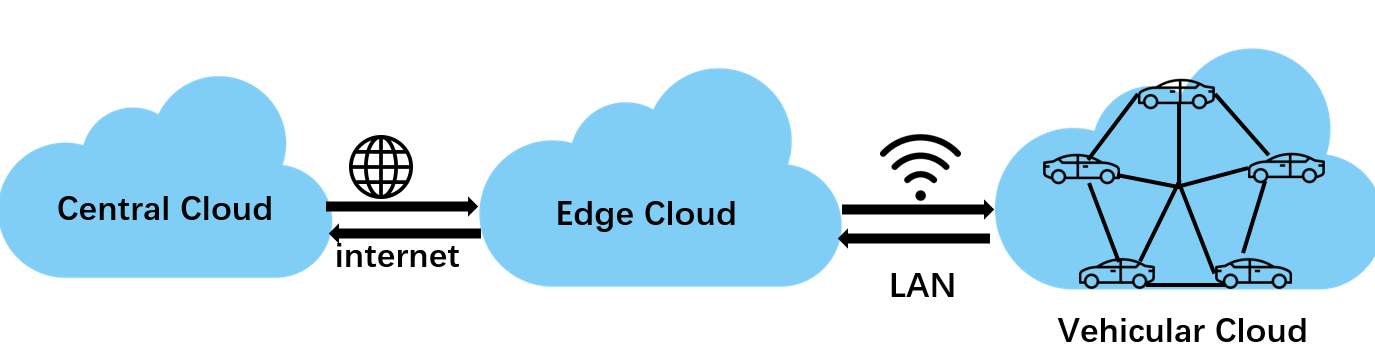
\includegraphics[width=0.80\textwidth]{pic2.png}
	\caption{Vehicular networks architecture}
	\label{cloud}
	
\end{figure*}

\subsection{Network Artechiture}
Similar to\cite{yu2013toward}, as shown in Fig.\ref{cloud}, the hierarchical architecture consisting vehicular cloud, edge cloud, and central cloud.

The task unloading process is as follows: first, the real-time traffic information is transmitted to the cloud server for analysis. The real-time information includes destination, current location, time, vehicle speed, and so on. After summarizing the data, the cloud server performs big data analysis to obtain the road congestion, and then infers the location information of the vehicle in a certain time period $T$ in the future, and returns the information to the edge cloud which is near the vehicle. The information includes the set of vehicles which are closed to the vehicle within the range of time $T$, these vehicles will participate in resource sharing.
Then, the edge cloud assigns tasks according to these information and divides the vehicles into providers and requesters, and the vehicles share resources at time slot $T$.
%约束


\begin{table}[]
	\centering
	\caption{Notations in This Paper}
	\begin{tabular}{|c|c|}
		\hline
		Parameter    &    Interpretation\\
		\hline
		%$P$	          & The provider      \\
		%$S_{it}$      & The provider $i$'s requester  \\
		%$V$          & The set of vehicles \\
		
		$T$	          & The resource sharing time   \\
		$C_{it}$      &   The CPU capacity    \\
		$r_i $   &   The workload of vehicle $i$ \\
		$r'_{jt} $ 	  &   The resource requester $j$ need    \\
		$M_{it}$      &   Millions Instructions Per Second(MIPS)   \\
		$\theta _i   $      &  Estimated parameters   \\
		
		$E^{blnc}_{it}$   &   Energy consumed by the vehicle $i$  \\
		
		$E^{rec}_i, E^{send}_i$ & Energy received or send by the vehicle $i$  \\
		
		
		\hline
	\end{tabular}
\end{table}

\subsection{Computation Model}
We define resource sharing time as $ \mathcal{T}=\{1, \ldots, T \}$. 
And the number of vehicles is defined as $N$. 
%, and denote the set of vehicles task as $\mathcal{N_{t}}=\{1_t, \ldots, N_t\}$ at each time slot $t$.
We use a tuple $J_{it} = \{r_ {it}, r'_ {it}, d_{it}\}$ to represent the task of vehicle $i$ at time slot $t$.
Tasks can be divided into tasks that can be offloaded and tasks that cannot be offloaded and must be executed locally. 
$r_ {it}$ is the number of instructions to complete the local task required by the vehicle $i$ at time slot $t$, 
$r'_ {it}$ is the number of instructions which  the vehicle $i$ task can offload to others at time slot $t$, 
and $d_{it}$ is the task's data size.

To facilitate the description of the model, we denote $\mathbf{X}_{t}=\left\{x_{i j}\right\} \in\{0,1\}^{N \times N}$ allocation matrix. If $x_{ij}=1$, it represents that vehicle $i$ performs the task of offloading vehicle $j$. Note that if $x_{ii}=1$, all tasks of vehicle $i$ are executed locally. 
%每一行代表做谁的任务, 每一列代表任务都给谁
%, and $\mathbf{X}_{t}=
%\left[\mathbf{x}_{1t}, \mathbf{x}_{2t}, \ldots, \mathbf{x}_{3t}, \ldots, \mathbf{x}_{Nt}\right]$, where $\mathbf{x}_{k}=\left[x_{1 k}, x_{2 k}, \ldots, x_{N k}\right]^{T}$. 

We characterize the computing capacity of vehicle $i$ by $C_ {it}$ at time $t$. When a vehicle is selected as a provider ($P$) at time $t$, the computing resources of all requester should be less than its computing capacity.
\begin{equation}
	\sum    \limits_{ j= 1} ^{N}
	{ x_{ij}^{t} \cdot  r'_{jt}} \le C_{it}, i = 1, \dots, N
	%,i \in P
\end{equation}
where $r'_ {jt} $is the computing resource that the requester needs at time slot $t$, $s_ {it}$ is the set of customers of the provider at time slot $t$. 
%For the convenience of description, the vector form is defined as $C_t = (C_{1t}, \dots ,C_{Nt})^T$, $R'_t =(r'_{1t}, \ldots , r'_{Nt})^T $ . 

A crucial step is how to quantify the computing resources. We regard the number of instructions that can be executed per unit time as the computing resources of a vehicle.The calculation capacity is defined based on the number of instructions executed per unit time (MIPS, $M_{it}$). 
\begin{equation}
	C_{it} = M_{it}   \cdot \Delta T 
	- r_{it}
	\label{cm}
\end{equation}
where $\Delta T$ is the duration of resource sharing, and is a smaller time scale than time of establishing vehicular network. After $\Delta T$ seconds, the offloading method changes
%

For a single core CPU, the number of instructions executed per unit time ($m_{it}$) and CPU frequency ($f_{it}$) have the following relationship:
\begin{equation}
	M_{it} = v_i \cdot f_{it} + \theta_i
	\label{mf}
\end{equation}
Where $v_ {i} $ and $\theta_ i$ are parameters to be estimated.
As a result, the CPU capacity $C_{it}$ in Equation (\ref{cm}) can be calculated following:
\begin{equation}
	C_{it} = (v_i \cdot f_{it} + \theta_i)   \times \Delta T 
	- r_{it}
	\label{cf}
\end{equation}
%To facilitate the description of the model, we denote $R'_t =(r'_{1t}, \ldots , r'_{Nt})^T $ 

%传输能耗
\subsection{Energy Consumption Model}
	When we consider the energy consumption, we divide it into two parts: (1) the energy required for calculation, (2) the energy required for send or receive. In this paper\cite{dysta}, the energy consumption of processor contain dynamic energy consumption $E ^{dynamic}$ and static energy consumption $E^{static}$. 
	And according to \cite{efv}\cite{vf}\cite{3940}\cite{4039}, the energy consumption is computed as follows:

\begin{equation}
	E=\lambda_{i} \cdot f_{it}^{3} \cdot \Delta T
	\label{ef}
\end{equation}
Where $f_ {it}$ is the frequency of the CPU in vehicle $i$ at time slot $t$. If a vehicle is selected as the requester(R), its frequency will decrease to $f^ \prime _ {it}$. Because its tasks are assigned, so the energy saved  is:
\begin{equation}
	E_{i}^{save}
	=( \lambda_{i} \cdot f_{it}^{3} -
	\lambda_{i} \cdot{f^{\prime}}_{i}^{3} ) \times \Delta T
	, 
	\forall i \in R
\end{equation}
%传输能耗

The transmission energy consumption is linear with the transmission time which depends on the ratio between the data size and the data transmission rate($b_{ij}$). 
\begin{equation}
	E = P_0 \cdot \frac{d_{it}}{b_{ij}}
\end{equation} 
where $P_0$ is the transmission power.

Maximum data transmission rate($b$) is given by Shannon theorem. 
\begin{equation}
	b_{ij} = W\log (1 + \text{SNR})
\end{equation}
where SNR is Signal-to-noise Ratio, and $W$ is the channel bandwidth.Because they are related to each actual channel, we regard it as a constant in this paper.

%每一行代表做谁的任务, 每一列代表任务都给谁
For each vehicle, the energy required for receiving information is:
\begin{equation}
	E_{i}^{r e c}=\sum_{j =1, j \ne i}^{N} x _{ij}^{t} \cdot P_0 \cdot \frac{d_{jt}}{W\log (1 + \text{SNR})}, 
	\quad  i = 1, \dots ,N
\end{equation}


%When the vehicle $i$ is selected as the provider, the energy required to receive the task is 
%Where $\omega_i$ is a parameter with estimation,Similarly, the energy required by the requester for transmission is
For each vehicle, the energy required for send information is:
\begin{equation}
	E_{i}^{send}=\sum_{i =1, i \ne j}^{N} x _{ij}^{t} \cdot P_0 \cdot \frac{d_{it}}{W\log (1 + SNR)},
	\quad  j = 1, \dots ,N
\end{equation}    
%定义 $E^{blnc}_{t}$ 为车辆在 $t$ 时刻的能量消耗, 该时刻, $i$ 为提供商时, 该时刻能量消耗为:

Define $E^{blnc}_ {t} $ is all the energy consumption of the vehicle in the time slot $t$ .
%The provider's energy consumption at this time is:
\begin{equation}
	\begin{aligned}
		%身为P 需要  接收
		E^{blnc} _{it}=
		%E^{ blnc } _{t-1} + 
		&\sum_{j=1, j \ne i}^{N} x _{ij}^{t} \cdot P_0 \cdot \frac{d_{jt}}{W\log (1 + \text{SNR})}   \\
		%E_{i}^{r e c}  
		+ &\sum_{j=1, , j \ne i}^{N} x _{ji}^{t} \cdot P_0 \cdot \frac{d_{it}}{W\log (1 + \text{SNR})}   \\
		+ &  \lambda_{i} \cdot f_{it}^{3} \cdot \Delta T
		, \quad i = 1, \dots ,N	
	\end{aligned}
\end{equation}
%In addition, when vehicle $i$ is the requester at this time $t$, , the total energy consumption is:
% \begin{equation}
	% send 
	%E^{blnc} _{it}=
	%\sum_{i=1}^{N} x _{ij} \cdot P_0 \cdot \frac{d_{jt}}{W\log (1 + SNR)} +
	%\lambda _i \cdot f '^ {3} _{it}\cdot \Delta T ,
	%\quad 
	%\forall i \in \mathcal{V} \backslash P
	%j = 1, \dots ,N
	% \end{equation}

	The objective of our algorithm is to minimize the quadratic power of energy over all vehicles. The goal is to balance and minimize energy consumption, because the square of the minimum drawing energy consumption.
\begin{equation}
	\min\sum \limits _{t=1} ^{T} \sum \limits _{i=1}^{N} (E^{blnc}_{it} )^ 2
\end{equation}
%Define it as vector form  
%and $F_t = (f_{1t}, \dots ,f_{Nt})^T$.



The problem can be formulated as:  
\begin{align}  		
	\min  \quad  &\sum \limits _{t=1} ^{T} \sum \limits _{i=1}^{N} (E^{blnc}_{it} )^ 2  \\
	\text{s.t.}   \quad   & 	    	E^{blnc} _{it}=
	%E^{ blnc } _{t-1} + 
	\sum \limits_{j=1,  j \ne i}^{N} x _{ij}^{t} \cdot P_0 \cdot \frac{d_{jt}}{W\log (1 + \text{SNR})}  \notag \\
	%E_{i}^{r e c}  
	&\quad \quad +\sum_{j=1 ,j \ne i }^{N} x _{ji}^{t} \cdot P_0 \cdot \frac{d_{it}}{W\log (1 + \text{SNR})}  \notag \\
	&\quad  \quad + \lambda_{i} \cdot f_{it}^{3} \cdot \Delta T
	,\quad i = 1, \dots ,N      \\
	%&\sum    \limits_{j \in S_{it}}
	%{r'_{jt}} <= C_{it}
	%,   i \in P   	       \\
	%& \mathbf{X}_{t} R'_{t} \le C  \\
	%&C_{it} = (v_i \cdot f'_{it} + \theta_i)   \times \Delta T 
	%- r_{it}    \\
	%& \Vert \mathbf{X}_{t} F_t \Vert_1  +\phi ^ T  \\
	%& C_{it} \ge 0           \\ 
	& \sum    _{ j= 1} ^{N}
	{ x_{ij}^{t} \cdot  r'_{jt}} \le C_{it}       \label{cons1}   \\
	& \sum  _{ i= 1} ^N x_{ij}^{t} 	\ge 1  \label{cons2} \\
	&     	f_{it} \ge 0         \label{cons3}\\
	&      x_{it}^{t} \in \{0,1\}	  \label{cons4}
\end{align} 

As mentioned above, the Equation(\ref{cons1}) shows all the amount of requested cannot exceed available capacity of vehicle $i$.
The Equation(\ref{cons2}) shows that the task of vehicle $i$ which can be offloaded must be executed whether by the vehicle $i$ or others. $f$ is the frequency and must be positive number. 

\subsection{Example}
\begin{equation*}
	\mathbf{X} = 
	\begin{bmatrix}		
		1  &  0  &  0   &0  &  0 \\
		0  &  1  &  0  &  0 &   0\\
		0  &  0  &  1 &   0  &  1\\
		0  &  0 &  0   & 1   & 0 \\
		0  &  0 &   0   & 0 &   0\\
	\end{bmatrix}
\end{equation*}

	The $\mathbf{X}$ is a example of allocation matrix. Vehicular set is \{A,B,C,D,E\}, the vehicle A, B and D don't assign and load other vehicular tasks, Therefore, they do not generate transmission energy consumption. And vehicle C execute the offloading task from vehicle E. And the sum of each column is greater than or equal to one.

\subsection{Constraints}
To ensure the Quality of Service(QoS) between the requester and provider, the following distance constraints need to be met:
\begin{equation}
	\min\limits_{ }
	l_{ij}^{t}<\delta
	,\quad
	i = 1,\dots,N,\forall x_{ij}^{t} =1
\end{equation}
where $l_ {ij}^{t}$ is the distance between vehicle $i$ and  $j$. If the constraint is not satisfied, the vehicle will exit resource sharing, and the $i$th row and the $i$th column of the allocation matrix are all set to zero while $x_{ii}^{t}=1$


%第四部分
\section{ALGORITHMS}

\begin{algorithm}[t]
	%设置算法编号
	%\renewcommand{\thealgocf}{3-1}
	\SetAlgoLined %显示end
	\caption{Greedy algorithm}%算法名字
	\label{greedy1}
	\KwIn{Vehicular real-time information}%输入参数
	%\KwOut{$ $}%输出
	%some description\; 
	%      '\;'   用于换行
	\While{true}{
		Update set of vehicles allocated to a vehicular network \;
		\For{t =1 to T/$\Delta T$}{
			\For{each edge server}{
				Establish vehicular network as controller  \;
				Run GA($Iterations, M, r', rloc, $) \;
				Every vehicle take participate in resource sharing according to the allocation matrix \;
			}
			
		}
		
		
	}
\end{algorithm} 
	We design a greedy algorithm \ref{greedy1} to minimize the energy consumption of all time slot. 
	For each moment, the central cloud returns the vehicles contained in each edge cloud and the time of participating in resource sharing, and all the edge cloud forms a vehicular cloud, then run genetic algorithm to minimize the energy consumption of a time slot. 
%伪代码
\begin{algorithm}[t]
	%设置算法编号
	%\renewcommand{\thealgocf}{3-1}
	\SetAlgoLined %显示end
	\caption{Genetic Algorithm}%算法名字
	\KwIn{input parameters $T, M, r', rloc, $}%输入参数
	\KwOut{$ \mathbf{X}, f, E$}%输出
	%\;用于换行
	$t = 0  $ \;
	Initialize $\mathbf{X}(0), f(0)$  \;
	
	
	
	\While{$t \textless T$}{
		Encoder $\mathbf{X}(t), f(t)$ \;
		\For{i = 1 to M}{
			Evaluate fitness  $P(ti) = -E_i$\;
			%\frac{-E_i}{\sum _{i=1}^{M} E_i   }
			%Select operation to $P(t)$ \;
			
			%Random a,b,c from $P(t)$  \;
			%Crossover operation to $P(t)$ \;
			
		}
		Eliminate fitness smaller individuals from $P(t)$ \;
		Replicate the fitness larger individuals  from $P(t)$ \;
		Divide the array composed of optimization variables into two. \;
		\For{i = 1 to M/2}{
			%
			Crossover operation to $P(t)$ \;
		}
		\For{i = 1 to M}{
			Mutation operation \;
		}
		%\For{i = 1 to M}{	$P(t+1) = P(t)$ \;}
		Decoder $\mathbf{X}(t), f(t)$ \;
		$t  \leftarrow t+1 $\;
	}%endwhile
	\For{i = 1 to N}{
		$E \leftarrow  E_i + E $
	}
	$\mathbf{X} =\mathbf{X}(t) , f = f(t)$ \;
	
	return $\mathbf{X}, f, E$ 
\end{algorithm}

Genetic algorithm is a adaptive heuristic optimization method, which is proposed by John Holland in 1970s\cite{gafirst}. Based on Darwin's theory of natural selection, it simulates the process of natural selection and reproduction to solve optimization problems. 
%Similarly to living organisms adapting to their environment over the generations, the solutions in the GA adapt to a fitness function over an iterative process using biology-like operators such as the crossovers of chromosomes, the mutations of genes and the inversions of genes. In recent years, the GA has been used for a wide range of applications such as the design of minimal phase digital filters [16] and the optimization of surface grinding process [17]. In this work, we use the GA to simulate the evolution of a population of trajectories adapting to the cost function defined in the previous section.
Similarly to individuals with favorable variation surviving , the solutions in the algorithm imitate the behavior of chromosomes, such as the mutations of genes and the crossovers of chromosomes.
In recently, the genetic algorithm has been used for real-time path planning\cite{gapathplan}, maximum coverage deployment in Wireless Sensor Networks\cite{GANetwork}, and intrusion detection\cite{GAIntrusionDetection}. 

In genetic algorithm, a population is composed of randomly generated solutions, and all individuals in the population are composed of encoded strings similar to chromosomes\cite{gaguocheng}.
Similar to natural selection, with the iteration, the diversity decreases, but the preserved individuals are excellent adaptive individuals. In other words, the preserved solutions are are locally optimal.

We develop a genetic algorithm called GA-Veh. 
Algorithm 1 is the pseudo-code of GA-Veh in our experiment. The algorithm has as input the vector of vehicles with their request size, $r'_i$, and their local workload $rloc $. The output consists of the allocation matrix $ \mathbf{X}_t$, the frequency $f_t$, and the energy consumption $E_t$ in the current time. 
At the initial stage of the algorithm, it will randomly generate a set of feasible solutions which is the first generation of chromosomes(Line2).
After that, $\mathbf{X}(t) $ and $ f(t)$is encoded as a string like a chromosome.
Then the fitness function is used to calculate the fitness degree for each chromosome(Line5-7), and the probability of each chromosome being selected in the next evolution is calculated according to the fitness degree(Line8).The chromosomes with lower fitness will be eliminated, and only the chromosomes with higher fitness will be retained(Line9).
Divide the individual into two parts at random(Line10).
A certain position of these two chromosomes is cut off and spliced together to generate a new chromosome.As a result, this new chromosome contains a certain number of genes of both father and mother(Line11-13).

Because the solution thus solved is closer to the local optimal solution, and there is no way to achieve the global optimal solution. In order to solve this problem, we need to introduce mutation(Line14-16). 
The next step is to decode the string to the original solution(Line17).
Finally we calculate all the energy consumption(Line20-22).






%第五部分 实验
\section{EXPERIMENT}
We set the parameters of the experiment and analyzed the result of the experiment in the section.

\subsection{The Setup}
As we all known, $U[x,y]$ is the uniform distribution between $x$ and $y$, and $N(x, y)$ is the normal distribution which  mean is $x$ and variance is $y$. 
We assume that the time which vehicles share their resource is $\Delta T = 10$ seconds, because of their limited space.

The Cortex-A57 processor is ARM's highest performing processor, designed to further mobile and enterprise computing applications\cite{a57}.
The Cortex-A57 has the frequency from 700 MHz to 1900 MHz. The frequency set is \{$700, 800, 900,,,1900$\}, as a result, there is only 13 frequency levels.
%We define three forms 

As is shown in Equation (\ref{mf}), the number of instructions is $M_{it} = v_i \cdot f_{it} + \theta_i$. 
And the CPU capacity in Equation (\ref{cf}) is $    	C_{it} = (v_i \cdot f_{it} + \theta_i)   \times \Delta T  - r_{it}$, 

We estimate the CPU capacity parameters $v_i, \theta_i$ is based on the analysis provided in \cite{vecman}, and the value is $7.683$ and $−4558.52$. 
After calculation, the maximum and minimum $M$  values are respectively $819, 10039$. 
%And the $r'_{it}$,  
The required computing resource $r_{it}$ for all tasks to execute workloads is uniformly drawn from [$ 820, 10000  $], and we assume that the task computing resource value $r'_{it}$ which vehicle $i$ can offload to others is $ U[200, r_{it}]$, because some subtask must be execute locally. 
In our experiment the size of data varies from 1MB to 10 MB. And we set the value of bandwith $d$ is 27Mb/s\cite{2017dsrc}
We have selected seven kinds of vehicle number to participate in resource sharing, which are$\{10,15, 20,25,30,35,40\}$. 

Our experiment are implemented in python and executed on an Intel Core i7 with 8 GB RAM.

%经典三线表格
\begin{table}[]
	\centering
	\caption{The values of parameters}
	\begin{tabular}{|c|c|}
		\hline
		Parameters    &    Values / Distribution   \\
		\hline
		
		$f_i$	          & $[700, 1900] $     \\
		$v_i$        &  $7.683$   \\
		$\theta $    & $-4558.52 $\\
		$\lambda$    &  $0.00125$ \\
		
		$\Delta T$      &   $1$   \\
		
		$r_{it}$     &     $ U[820, 10000]$   \\
		$r'_{it} $  &   $ U[200, r_{it}]$ \\
		
		$P_0$      &   $0.2$   \\
		%	$W\log (1 + \text{SNR}) $      &   $27$   \\
		$W$ & 10 MHz \\
		\text{SNR} & 677\\
		\hline
	\end{tabular}
\end{table}

\subsection{Performance Metrics}
The performance of our experiment is the percentage of energy saving,which is define as follows:
\begin{equation}
	P = 100 \cdot 
	( 1-
	\frac{
		\sum \limits _{t=1} ^{T} \sum \limits _{i} E^{blnc}_{it}   }{E_{loc}})
\end{equation}
where $E_{loc}$ is the energy consumed by local task execution. 

In order to reflect the fairness of our framework, we define the fairness coefficient ($FC$) based on the standard deviation
As with the standard deviation, the smaller the value the greater the fairness. $FC$ is define as follows.
%A lower value of CV means a more fair distribution of requests.
\begin{equation}
	FC=\frac{\sqrt{\frac{1}{N} \sum_{i=1}^{N}\left(E_{it}^{b l n c}-\bar{E}\right)^{2}}}{\bar{E}}
\end{equation}

\subsection{Experimental Results}
%图片-能耗
\begin{figure}[htbp]
	%居中
	\centering
	%\includegraphics[width=2.5in]{Autoencoder1}
	%占据0.8宽度
	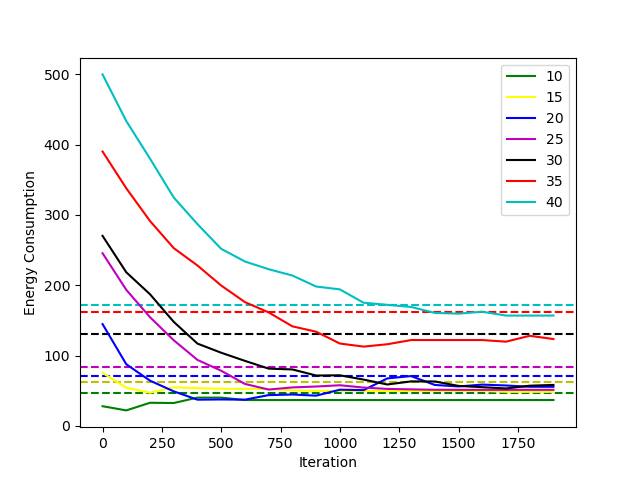
\includegraphics[width=0.40\textwidth]{energy.png}
	%图片名称
	\caption{Energy Consumption}
	\label{energy}
\end{figure}
In Fig.\ref{energy}, the dotted line is the energy consumed by local execution. 
%In general, the more vehicles, the more iterations are required. 
We can see that when the number of vehicles is 10, the algorithm can get good results by running a few times. While the number of vehicles is 20, it takes 350 iterations to get a better result. 
And when the number of vehicles is 30, the reduction rate of energy consumption is faster before 750 iterations, and will be significantly slower after 750 iterations . 
Almost no energy saving when the number of vehicles is 40. 
%And the number of vehicles is 70, that point is 1500.
We can conclude that with the increase of the number of vehicles, the number of iterations is also increasing. 
Therefore, when we run the algorithm on the edge server, we need to adjust the number of iterations reasonably as the number of vehicles changes. 
%图片运行时间
\begin{figure}[htbp]
	%居中
	\centering
	%\includegraphics[width=2.5in]{Autoencoder1}
	%占据0.8宽度
	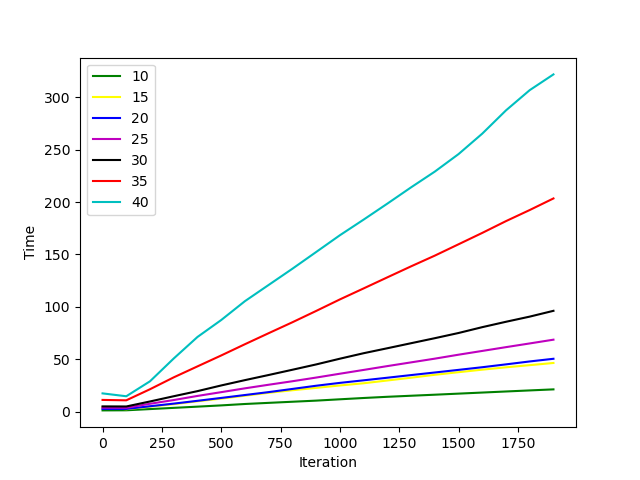
\includegraphics[width=0.40\textwidth]{time.png}
	%图片名称
	\caption{Experimental running time}
	\label{time}
\end{figure}

In Fig.\ref{time}, after 100 iterations, the running time and the number of iterations show a linear relationship. However, when the number of iterations is fixed, the relationship between time and vehicle is not linear. 
As Fig.\ref{fc} shows, we can see that with the increase of vehicles, the balance of vehicle energy consumption increases first and then decreases. 
As Fig.\ref{p} shows, when the number of vehicles is 10 and 20, our system can save half of the energy consumption, but when the number of vehicles is 25, only 25\% can be saved, and when the number of vehicles is 40, almost no savings. 
%图片-度量
\begin{figure}[htbp]
	\centering
	\subfigure[The values of FC]{
		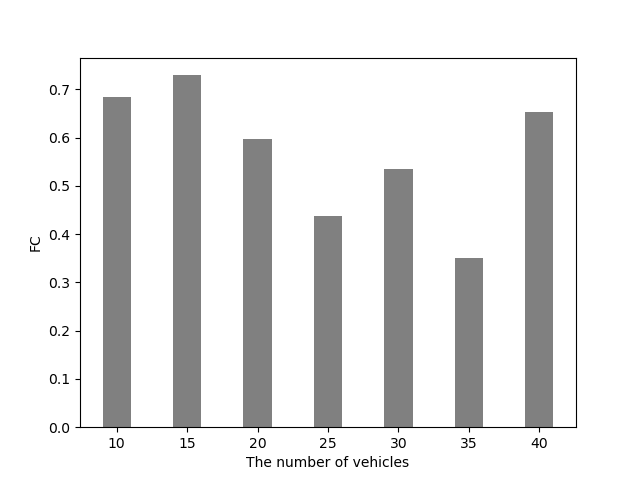
\includegraphics[scale=0.4]{FC.png} \label{fc}
	}
	\quad
	\subfigure[The values of P]{
		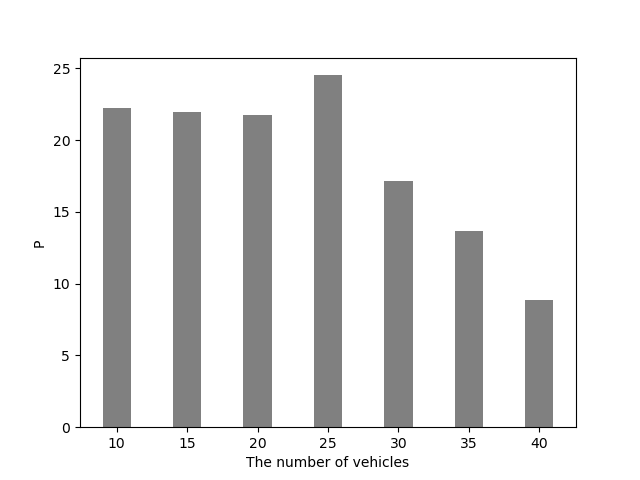
\includegraphics[scale=0.4]{P.png} \label{p} 
	}
	\caption{Performance metrics}
\end{figure}


%结果正文
%\subsection{Conclusion}

Considering the performance measurement, energy consumption and time, it is appropriate to choose 25 vehicles to participate in resource sharing. 
\section{CONCLUSIONS AND FUTURE}
In this paper, we proposed task offloading based on genetic algorithm for electric smart vehicle. We evaluate the performance of the algorithm through simulation experiments. 
Experimental results show that our algorithm can achieve the goal of energy conservation. 
In the future research, we plan to establish the relationship between the data size and the number of instructions and consider the deadline constraints.




%参考文献

%\bibliography{ref}

\printbibliography

\end{document}
